\documentclass[margin=0mm,tikz]{standalone}

\usepackage{tikz}
\usepackage{xcolor}
%\usepackage{mathtools}
%\usepackage{stackengine}
\usepackage{amsmath}

\usetikzlibrary{positioning}
\usetikzlibrary{calc}
\usetikzlibrary{arrows.meta}

\pgfdeclarelayer{background}
\pgfsetlayers{background,main}

% -----------------------
% colors
% -----------------------
\definecolor{losscolor}{RGB}{175, 0, 23}
\definecolor{convblockcolor}{RGB}{0, 93, 157}
\definecolor{downscalecolor}{RGB}{48, 11, 213}
\definecolor{upscalecolor}{RGB}{11, 176, 213}
\definecolor{forwardcolor}{RGB}{100, 100, 100}
\definecolor{skipcolor}{RGB}{218, 138, 0}
\definecolor{operatorcolor}{RGB}{136, 150, 186}
\definecolor{reccolor}{RGB}{113, 0, 162}
\definecolor{catcolor}{RGB}{255, 0, 0}


% Set background color
%\pagecolor{white}

% -----------------------
% styles
% -----------------------

\tikzstyle{conv} = [-{Latex[length=6pt, width=10pt]}, line width=3pt, convcolor]
\tikzstyle{convblock} = [-{Latex[length=6pt, width=10pt]}, line width=3pt, convblockcolor]
\tikzstyle{downscale} = [-{Latex[length=6pt, width=10pt]}, line width=3pt, downscalecolor]
\tikzstyle{upscale} = [-{Latex[length=6pt, width=10pt]}, line width=3pt, upscalecolor]
\tikzstyle{forward} = [-{Latex[length=2pt, width=4pt]}, line width=1pt, forwardcolor]
\tikzstyle{skip} = [-{Latex[length=3pt, width=5pt]}, line width=2pt, skipcolor]
\tikzstyle{rec} = [-{Latex[length=6pt, width=10pt]}, line width=3pt, reccolor]
\tikzstyle{cat} = [dashed, line width=1pt, catcolor]

\tikzstyle{model} = [draw=convblockcolor!80!black, thick, top color=convblockcolor!10!white, bottom color=convblockcolor!20!white]  % fill=white!95!black

\begin{document}
	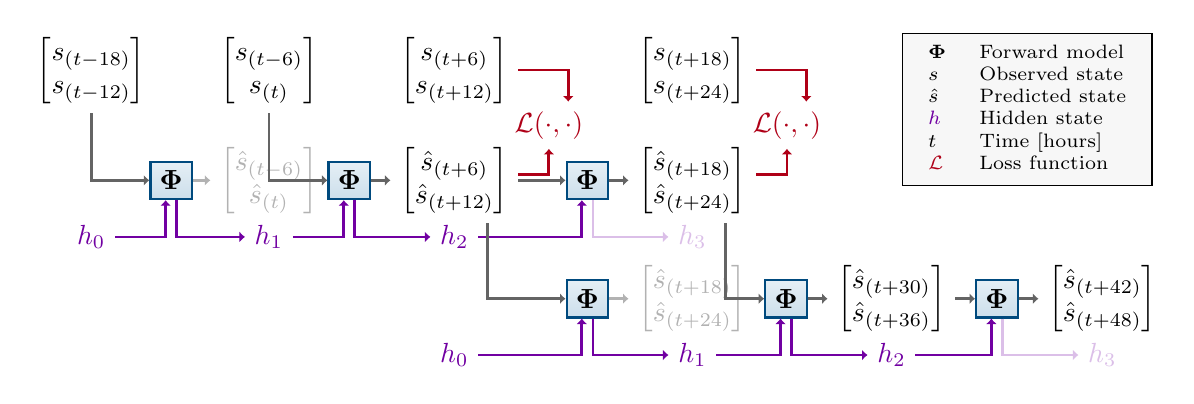
\begin{tikzpicture}[node distance=0.4cm]
		
		%
		% Ground Truth
		\node (s_m18_m12) {$\begin{bmatrix}	s_{(t-18)} \\ s_{(t-12)} \end{bmatrix}$};
		\node [right=0.7cm of s_m18_m12] (s_m6_0) {$\begin{bmatrix}	s_{(t-6)} \\ s_{(t)} \end{bmatrix}$};
		\node [right=0.8cm of s_m6_0] (s_p6_p12) {$\begin{bmatrix}	s_{(t+6)} \\ s_{(t+12)} \end{bmatrix}$};
		\node [right=1.4cm of s_p6_p12] (s_p18_p24) {$\begin{bmatrix}	s_{(t+18)} \\ s_{(t+24)} \end{bmatrix}$};
		
		%
		% First cycle (0h to 24h)
		
		% First model call
		\node [below=1.3cm of s_m18_m12, reccolor] (h0_0) {$h_0$};
		\node [model] at ([yshift=-1.4cm]$(s_m18_m12)!0.45!(s_m6_0)$)(phi0_0h) {$\boldsymbol{\Phi}$};
		\node [white!70!black] at (s_m6_0 |- phi0_0h) (sh_m6_0) {$\begin{bmatrix}	\hat{s}_{(t-6)} \\ \hat{s}_{(t)} \end{bmatrix}$};
		\node [reccolor] at (h0_0 -| sh_m6_0) (h0_1) {$h_1$};
		
		\draw [forward] (s_m18_m12.south) -- (s_m18_m12 |- phi0_0h) -- (phi0_0h);
		\draw [forward, reccolor] (h0_0.east) -- ([xshift=-2]h0_0 -| phi0_0h) -- ([xshift=-2]phi0_0h.south);
		\draw [forward, white!70!black] (phi0_0h) -- (sh_m6_0);
		\draw [forward, reccolor] ([xshift=2pt]phi0_0h.south) -- ([xshift=2pt]h0_0 -| phi0_0h) -- (h0_1);
		
		% Second model call
		\node [right=0.0cm of sh_m6_0, model] (phi0_12h) {$\boldsymbol{\Phi}$};
		\node at (s_p6_p12 |- phi0_12h) (sh_p6_p12) {$\begin{bmatrix} \hat{s}_{(t+6)} \\ \hat{s}_{(t+12)} \end{bmatrix}$};
		\node [reccolor] at (h0_1 -| sh_p6_p12) (h0_2) {$h_2$};
		
		\draw [forward] (s_m6_0.south) -- (s_m6_0 |- phi0_12h) -- (phi0_12h);
		\draw [forward, reccolor] (h0_1.east) -- ([xshift=-2]h0_1 -| phi0_12h) -- ([xshift=-2]phi0_12h.south);
		\draw [forward] (phi0_12h) -- (sh_p6_p12);
		\draw [forward, reccolor] ([xshift=2pt]phi0_12h.south) -- ([xshift=2pt]h0_1 -| phi0_12h) -- (h0_2);
		
		% Third model call
		\node [right=0.6cm of  sh_p6_p12, model] (phi0_24h) {$\boldsymbol{\Phi}$};
		\node at (s_p18_p24 |- phi0_24h) (sh0_p18_p24) {$\begin{bmatrix} \hat{s}_{(t+18)} \\ \hat{s}_{(t+24)} \end{bmatrix}$};
		\node [white!75!reccolor] at (h0_2 -| sh0_p18_p24) (h0_3) {$h_3$};
		
		\draw [forward] (sh_p6_p12) -- (phi0_24h);
		\draw [forward, reccolor] (h0_2.east) -- ([xshift=-2]h0_2 -| phi0_24h) -- ([xshift=-2]phi0_24h.south);
		\draw [forward] (phi0_24h) -- (sh0_p18_p24);
		\draw [forward, white!75!reccolor] ([xshift=2pt]phi0_24h.south) -- ([xshift=2pt]h0_2 -| phi0_24h) -- (h0_3);
		
		% Loss
		\node [losscolor] at ([xshift=1.2cm]$(s_p6_p12)!0.5!(sh_p6_p12)$) (loss1) {$\mathcal{L}(\cdot, \cdot)$};
		\draw [forward, losscolor] ([yshift=2]sh_p6_p12.east) -- ([yshift=2pt]sh_p6_p12 -| loss1) -- (loss1);
		\draw [forward, losscolor] (s_p6_p12) -- ([xshift=7]s_p6_p12 -| loss1) -- ([xshift=7pt]loss1.north);
		
		\node [losscolor] at ([xshift=1.2cm]$(s_p18_p24)!0.5!(sh0_p18_p24)$) (loss2) {$\mathcal{L}(\cdot, \cdot)$};
		\draw [forward, losscolor] ([yshift=2]sh0_p18_p24.east) -- ([yshift=2pt]sh0_p18_p24 -| loss2) -- (loss2);
		\draw [forward, losscolor] (s_p18_p24) -- ([xshift=7]s_p18_p24 -| loss2) -- ([xshift=7pt]loss2.north);
		
		%
		% Second cycle (24h to 48h)
		
		% First model call
		\node [below=1.4cm of sh_p6_p12, reccolor] (h1_0) {$h_0$};
		\node [below=of  phi0_24h, yshift=-0.6cm, model] (phi1_0h) {$\boldsymbol{\Phi}$};
		\node [white!70!black] at (sh0_p18_p24 |- phi1_0h) (sh1_p18_p24) {$\begin{bmatrix}	\hat{s}_{(t+18)} \\ \hat{s}_{(t+24)} \end{bmatrix}$};
		\node [reccolor] at (h1_0 -| sh1_p18_p24) (h1_1) {$h_1$};
		
		\draw [forward] ([xshift=12pt]sh_p6_p12.south) -- ([xshift=12pt]sh_p6_p12 |- phi1_0h) -- (phi1_0h);
		\draw [forward, reccolor] (h1_0.east) -- ([xshift=-2]h1_0 -| phi1_0h) -- ([xshift=-2]phi1_0h.south);
		\draw [forward, white!70!black] (phi1_0h) -- (sh1_p18_p24);
		\draw [forward, reccolor] ([xshift=2pt]phi1_0h.south) -- ([xshift=2pt]h1_0 -| phi1_0h) -- (h1_1);
		
		% Second model call
		\node [right=0.1cm of sh1_p18_p24, model] (phi1_12h) {$\boldsymbol{\Phi}$};
		\node [right=0.25cm of phi1_12h] (sh_p30_p36) {$\begin{bmatrix} \hat{s}_{(t+30)} \\ \hat{s}_{(t+36)} \end{bmatrix}$};
		\node [reccolor] at (h1_1 -| sh_p30_p36) (h1_2) {$h_2$};
		
		\draw [forward] ([xshift=12pt]sh0_p18_p24.south) -- ([xshift=12pt]sh0_p18_p24 |- phi1_12h) -- (phi1_12h);
		\draw [forward, reccolor] (h1_1.east) -- ([xshift=-2]h1_1 -| phi1_12h) -- ([xshift=-2]phi1_12h.south);
		\draw [forward] (phi1_12h) -- (sh_p30_p36);
		\draw [forward, reccolor] ([xshift=2pt]phi1_12h.south) -- ([xshift=2pt]h1_1 -| phi1_12h) -- (h1_2);
		
		% Third model call
		\node [right=0.25cm of  sh_p30_p36, model] (phi1_24h) {$\boldsymbol{\Phi}$};
		\node [right=0.25cm of phi1_24h] (sh_p42_p48) {$\begin{bmatrix} \hat{s}_{(t+42)} \\ \hat{s}_{(t+48)} \end{bmatrix}$};
		\node [white!75!reccolor] at (h1_2 -| sh_p42_p48) (h1_3) {$h_3$};
		
		\draw [forward] (sh_p30_p36) -- (phi1_24h);
		\draw [forward, reccolor] (h1_2.east) -- ([xshift=-2]h1_2 -| phi1_24h) -- ([xshift=-2]phi1_24h.south);
		\draw [forward] (phi1_24h) -- (sh_p42_p48);
		\draw [forward, white!75!reccolor] ([xshift=2pt]phi1_24h.south) -- ([xshift=2pt]h1_2 -| phi1_24h) -- (h1_3);
		
		%
		% Legend		
		\node [right=of loss2 , yshift=0.2cm, xshift=0.5cm, draw, fill=white!97!black] (table) {
			\scriptsize
			\begin{tabular}{ll} 
				$\boldsymbol{\Phi}$ & Forward model \\
				$s$ & Observed state \\
				$\hat{s}$ & Predicted state \\
				\color{reccolor}$h$ & Hidden state \\
				$t$ & Time [hours] \\
				\color{losscolor}$\mathcal{L}$ & Loss function
			\end{tabular}
		};
	
	\end{tikzpicture}
\end{document}